

\section{Use case: Threads and replies}
	\subsection{Use case diagram}
	\begin{description}
		\item[Use case diagram for threads.] 
	\end{description}
	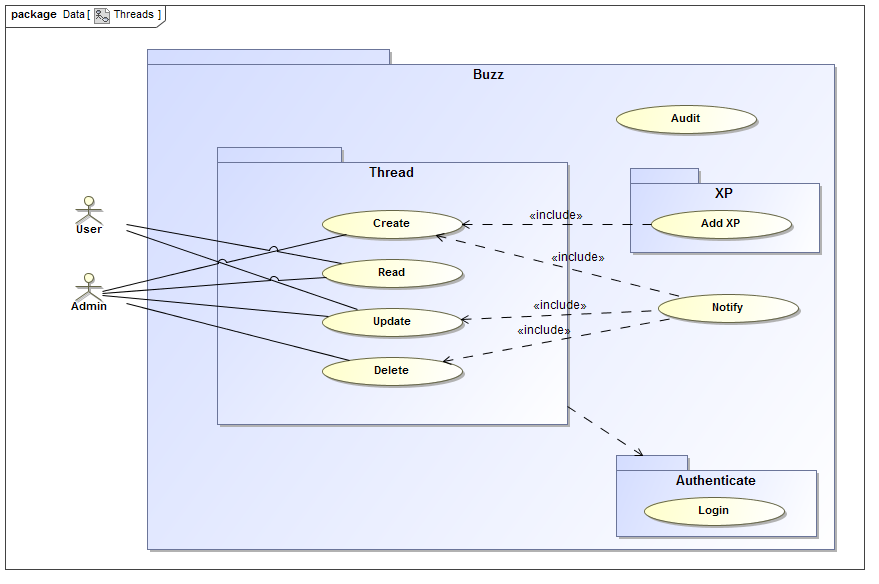
\includegraphics[width=\textwidth]{Threads}
\newpage
		\begin{description}
			\item[Use case diagram for replies.] 
		\end{description}
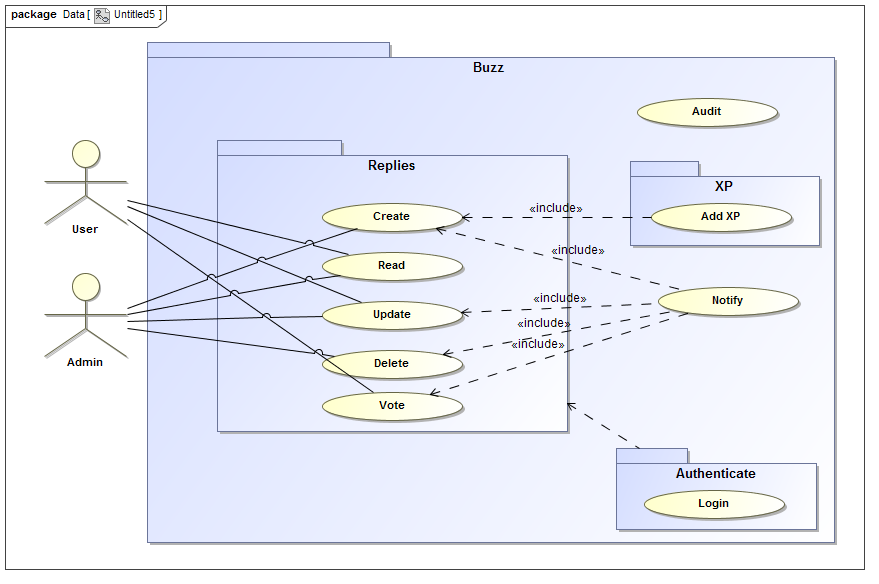
\includegraphics[width=\textwidth]{Replies}
	
	\subsection{Short description}
	\begin{description}
		\item[Above diagrams depicts the relationships between different components for ]
		 \item[the thread and reply systems within Buzz.] 
	\end{description}
	\subsection{Use cases}


\begin{table}
\begin{tabularx}{\textwidth}{|>{\setlength\hsize{0.5\hsize}\setlength\linewidth{\hsize}}X|>{\setlength\hsize{.8\hsize}\setlength\linewidth{\hsize}}X|>{\setlength\hsize{.9\hsize}\setlength\linewidth{\hsize}}X|>{\setlength\hsize{0.8\hsize}\setlength\linewidth{\hsize}}X|}
\hline
	\multicolumn{4}{|c|}{\textbf{Use cases for: Threads and Replies}}\\
\hline
	\paragraph{Use Case} & \paragraph{Precondition} & \paragraph{Post-condition} & \paragraph{Description} \\
\hline
	\paragraph{Create Thread}
&
\begin{itemize}
	\item Creator must be authenticated and  logged in
	\item Creator must have the necessary privileges to create a topic in the current space
	\item Creator must belong to a group
	
	
\end{itemize} &
\begin{itemize}
\item	Thread contains a subject or title
\item	Thread contains a clear short description 
\item	Thread shows the author
\item	Thread shows status(Published /Unpublished)
\item	Thread contains descriptive tags
\item	Thread shows total replies (if any available)
\item	Thread belongs to a category
\item	Thread has a valid date
\item	Thread allows for users to rate it
\item Thread is saved to database
\item All relevant users are notified of the existence of the thread
\item Creator of thread recieves Xp

\end{itemize} &
	\paragraph{Creates a thread within a space with the neccesary information}
\\
\hline
	\paragraph{Create Reply}
	&
	\begin{itemize}
\item	User  must be authenticated and  logged in
\item	User must belong to a group
\item	User must be able to participate in threads within current space
\item	A thread must exist
	
		
		
	\end{itemize} &
	\begin{itemize}
\item Reply post is linked to the right thread
\item Reply is in correct format
\item Reply is in correct format
\item Reply is saved to database
	\item All relevant users are notified that a reply has been posted

	\end{itemize} &
	\paragraph{Creates a reply thats part of a thread}
	\\
	\hline
		\paragraph{Delete Thread}
		&
		\begin{itemize}
			\item	User  must be authenticated and  logged in
			\item	User must belong to a group
			\item	A thread must exist
			\item  user must have the necessary privileges(or Xp) to delete a thread in the current space
			
			
			
		\end{itemize} &
		\begin{itemize}
			\item Thread is deleted
			\item All relevant users are notified that the thread is deleted
		
			
		\end{itemize} &
		\paragraph{A thread is deleted}
		\\
	\hline
\end{tabularx}
\end{table}
\newpage
\begin{table}
	\begin{tabularx}{\textwidth}{|>{\setlength\hsize{0.5\hsize}\setlength\linewidth{\hsize}}X|>{\setlength\hsize{.8\hsize}\setlength\linewidth{\hsize}}X|>{\setlength\hsize{.9\hsize}\setlength\linewidth{\hsize}}X|>{\setlength\hsize{0.8\hsize}\setlength\linewidth{\hsize}}X|}
		\hline
		\multicolumn{4}{|c|}{\textbf{Use cases for: Threads and Replies}}\\
		\hline
		\paragraph{Use Case} & \paragraph{Precondition} & \paragraph{Post-condition} & \paragraph{Description} \\
		\hline
		\paragraph{Delete Reply}
		&
		\begin{itemize}
				\item	User  must be authenticated and  logged in
				\item	User must belong to a group
				\item	A thread must exist
				\item  user must have the necessary privileges(or Xp) to delete a thread in the current space
				
			
			
		\end{itemize} &
		\begin{itemize}
			\item Reply is deleted
				\item All relevant users are notified that a reply has been deleted
				
			
			
			
		\end{itemize} &
		\paragraph{Delete a reply}
		\\
			\hline
			\paragraph{Update Thread}
			&
			\begin{itemize}
				\item	User  must be authenticated and  logged in
				\item	User must belong to a group
				\item	A thread must exist
				\item  user must have the necessary privileges(or Xp) to update a thread in the current space
				
				
				
			\end{itemize} &
			\begin{itemize}
				\item Thread is updated
				\item Thread is saved to the database
						\item All relevant users are notified that an update to a thread has been made
						
				
				
				
			\end{itemize} &
			\paragraph{User updates a thread}
			\\
			\hline
			
				\paragraph{Update Reply}
				&
				\begin{itemize}
					\item	User  must be authenticated and  logged in
					\item	User must belong to a group
					\item	A thread must exist
					\item  user must have the necessary privileges(or Xp) to update a reply in the current space
					
					
					
				\end{itemize} &
				\begin{itemize}
					\item Thread is updated
					\item Thread is saved to the database
						\item All relevant users are notified that an update to a reply has been made
					
					
					
				\end{itemize} &
				\paragraph{User updates a reply}
				\\
				\hline
	

	\end{tabularx}
\end{table}
\newpage
\begin{table}
	\begin{tabularx}{\textwidth}{|>{\setlength\hsize{0.5\hsize}\setlength\linewidth{\hsize}}X|>{\setlength\hsize{.8\hsize}\setlength\linewidth{\hsize}}X|>{\setlength\hsize{.9\hsize}\setlength\linewidth{\hsize}}X|>{\setlength\hsize{0.8\hsize}\setlength\linewidth{\hsize}}X|}
		\hline
		\multicolumn{4}{|c|}{\textbf{Use cases for: Threads and Replies}}\\
		\hline
		\paragraph{Use Case} & \paragraph{Precondition} & \paragraph{Post-condition} & \paragraph{Description} \\
		\hline
	
		\paragraph{Read a Thread}
		&
		\begin{itemize}
			\item	User  must be authenticated and  logged in
			\item	User must belong to a group
			\item	User must be able to participate in threads within current space
			\item	A thread must exist
			
			
			
		\end{itemize} &
		\begin{itemize}
		\item Thread status is updated to read for the current user
			
		\end{itemize} &
		\paragraph{User reads a thread}
		\\
		\hline
		\paragraph{Read a reply}
		&
		\begin{itemize}
			\item	User  must be authenticated and  logged in
			\item	User must be able to participate in threads within current space
			\item	A thread must exist
		
			
			
		\end{itemize} &
		\begin{itemize}
	\item Reply status is updated to read for the current user
			
			
		\end{itemize} &
		\paragraph{User reads a reply}
		\\
			\hline
			\paragraph{Vote}
			&
			\begin{itemize}
				\item	User  must be authenticated and  logged in
				\item	User must be able to participate in threads and replies within current space
		
				
				
			\end{itemize} &
			\begin{itemize}
				\item A vote has been made to a thread or reply.
				
				
			\end{itemize} &
			\paragraph{Users vote for threads and replies based on the relevance of the content}
			\\
			\hline
	\end{tabularx}
\end{table}
